\newpage
\section{Teilversuch 3: Bestimmung der Vergrößerung des Foldscopes}
	\begin{tabularx}{\textwidth}{l p{1mm} X}
		\toprule
		\tou{Versuchsziel} && Bestimmung der Vergrößerung des Foldscopes \\
		\tou{Messmethode} && Samsung Galaxy S10e (SM-G970F) mit der $f/1.5$-$2.4$, $\SI{26}{\milli\meter}$ Kamera, GIMP \\
		\bottomrule
	\end{tabularx}
	\subsection{Überlegungen}
		Es ist leider nicht möglich, genaue Messungen mit der Augen durchzuführen, also müssen wir ein Analogon zu den Augen herausfinden. Ein natürliches Analogon wäre eine Smartphone Kamera, besonders wenn wir schon ein Montiermechanismus mit der dritten Magnetkoppler haben. 

		\begin{center}
			\vspace{10pt}
			\renewcommand*{\arraystretch}{1.5}
			\begin{tabularx}{0.9\textwidth}{l X}
				\toprule
				Ähnlichkeiten & Es ist ein reelles Bild auf einem Sensor (Nezthaut vs. CCD) abgebildet. \\[-0.5em]
				& Der Brennpunkt kann variert werden, um auf Gegenständen in unterschiedlicher Entfernung zu fokussieren. \\
				Unterscheidung & Der Mechanismus, mit dem man die Brennweite ändert. \\
				\bottomrule
			\end{tabularx}
			\vspace{10pt}
		\end{center}

		Im menschlichen Auge ist die Linse mit Muskeln verförmt, um das Bild auf dem Netzhaut im Fokus zu bringen. 

		Da die Kamera öffensichtlich keine Linsen verförmen können, ist das Mechanismus normarlerweise eine(ein) bewegliche(s) Linse(nsystem). Jedes optische System lässt sich als eine dünne Linse mit zwei Hauptebenen (und zusätzliche Translation) dargestellt werden, also kann man die Kamera problemlos als eine Linse betrachten \citep{saleh_14_2019}. 

		\begin{wrapfigure}{r}{0.4\textwidth}
			\centering
			\vspace{-5pt}
			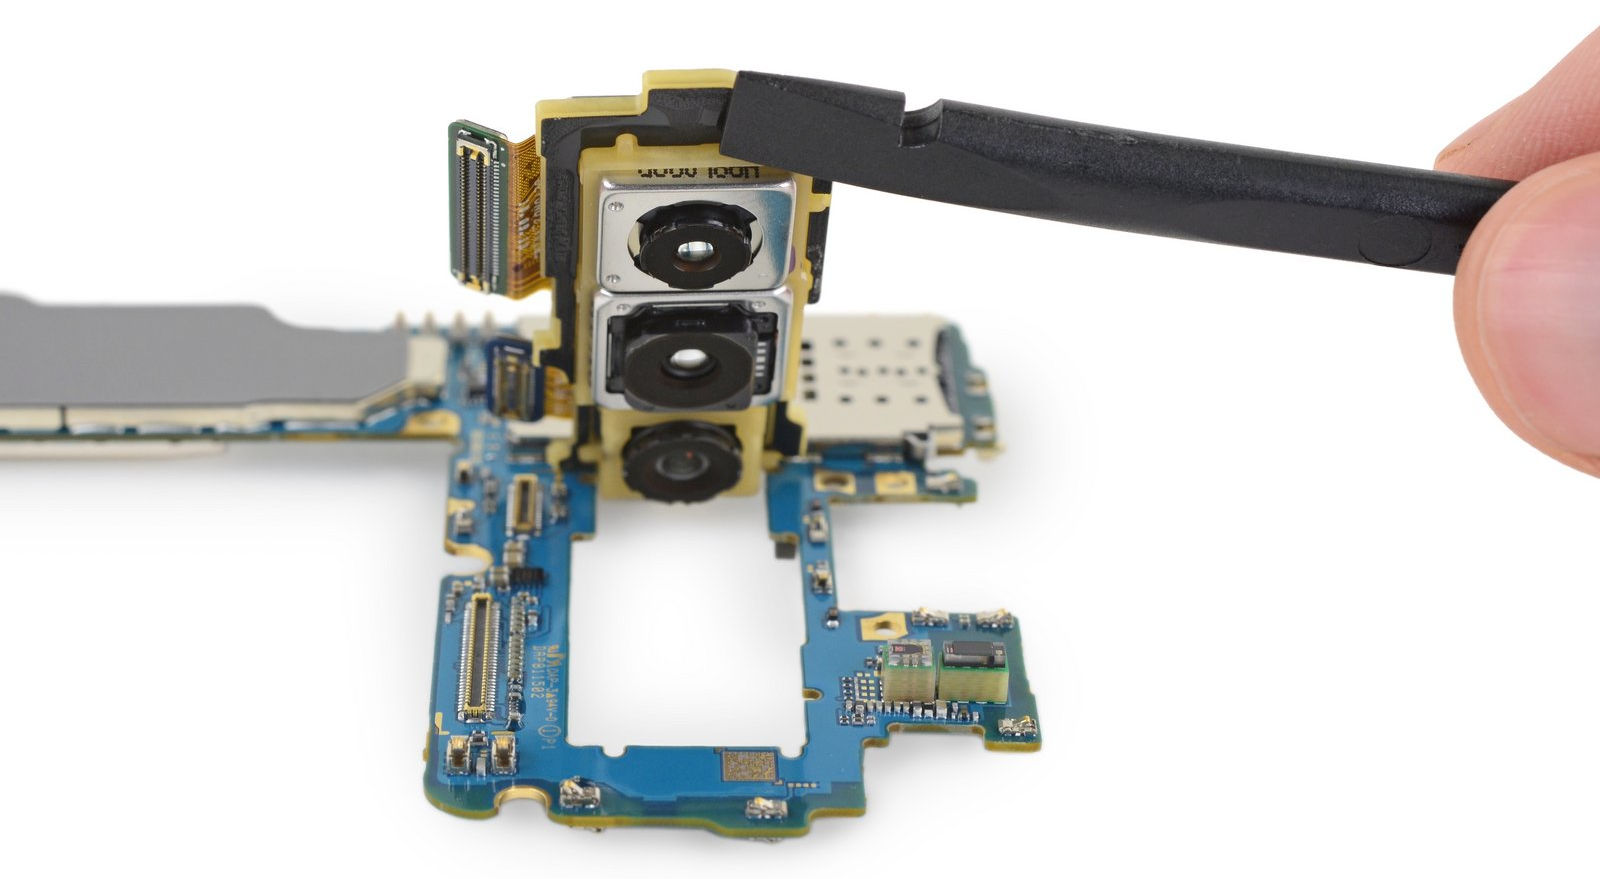
\includegraphics[width=0.4\textwidth]{images/camera.jpg}
			\caption{Kameramodul des Samsung Galaxy S10, das ähnliche Kameramodule wie das Samsung Galaxy S10e verwendet. Bild aus \textit{ifixit.com}.}
			\vspace{5pt}
			\label{fig:ifixit}
			\vspace{-20pt}
		\end{wrapfigure}
		Wir wissen aber nicht, ob die Hauptebene der Kamera sich während der Fokussierung so verschiebt, dass die Gegenstandsweite zu groß verändert oder wie groß die mögliche Translation ist, wenn man das optisches System als eine dünne Linse betrachtet. Wenn solche Probleme nicht vernächlassigt werden kann, dann ist die Kamera keinen guten Ersatz für das Auge.
		
		Nach einer schnellen Suche findet man aber aus der iFixit Seite der Samsung Galaxy S10e\footnote{\url{https://www.ifixit.com/Teardown/Samsung+Galaxy+S10+and+S10e+Teardown/120331}} ein Foto vom Kameramodul des Smartphones (Abbildung \ref{fig:ifixit})
		
		Das Kameramodul ist also nicht größer als einige Millimeter. 

		Wir vermuten somit, dass die Verschiebung der Hauptebene ebenfalls von einiger Millimeter begrenzt ist und deswegen im unseren Versuch keine große Rolle spielt. Wir müssen bei der Bestimmung der Gegenstandsweite sowieso schon mit einem Fehler von mindestens $\pm \SI{1}{\milli\meter}$ rechnen. 

		Eine Smartphonekamera ist somit eine gute Annährung für das menschliche Auge.
	\subsection{Durchführung}
		Um die Vergrößerung zu bestimmen ist die Breite einer Bleistiftmine als Maßstab verwendet, da diese im Sichtfeld des Foldscopes gut passt. Diese Bleistiftmine ist eine \SI{0.5}{\milli\meter} 2B Polymer Bleistiftmine, die von der \textit{Pilot Corporation} hergestellt ist. 

		\vspace{0.5\baselineskip}
		\underline{\large\textit{Bloße Augen}}
		\vspace{0.5\baselineskip}

			\begin{figure}[H]
				\centering
				\begin{subfigure}[b]{0.48\textwidth}
					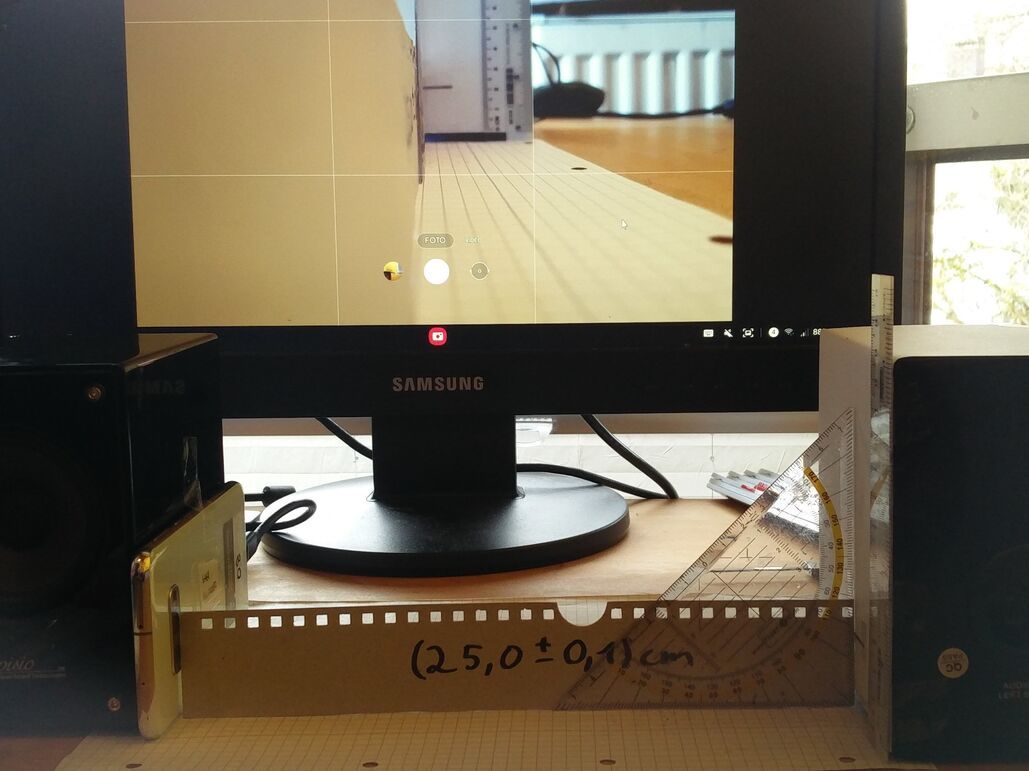
\includegraphics[width=\textwidth]{images/tv3/tv3-aufbau-01.jpg}
					\caption{Ansicht von Vorne}
				\end{subfigure}
				\hspace{5pt}
				\begin{subfigure}[b]{0.48\textwidth}
					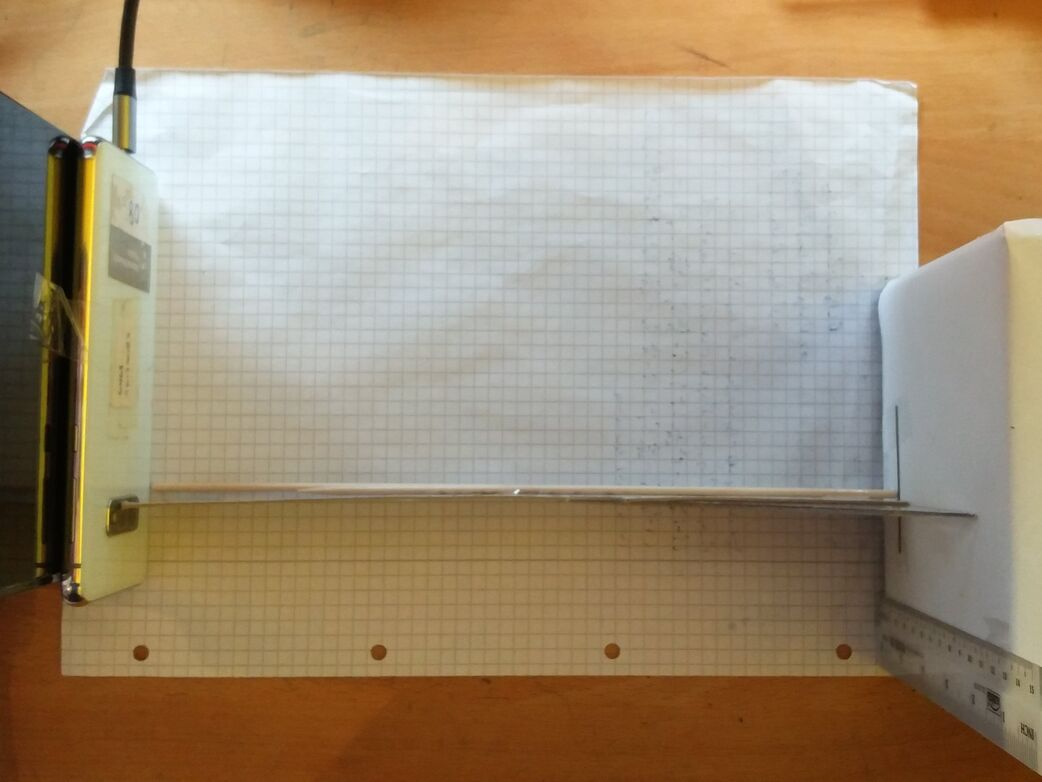
\includegraphics[width=\textwidth]{images/tv3/tv3-aufbau-02.jpg}
					\caption{Ansicht von Oben}
				\end{subfigure}
				\caption{Aufbau für bloße Augen}
				\label{fig:tv3-fern-aufbau}
				\vspace{-10pt}
			\end{figure}
			Für die bloße Augen wurden zwei Lautsprecherboxen als Befestigungsfläche verwendet. Die Rechtwinkligkeit dieser Oberflächen wurde mit einem Geodreieck überprüft. Um den Abstand zwischen der beiden Lautsprecherboxen einzustellen, wurde ein Maßstab der Länge \SI{25.0(1)}{\centi\meter} (deutliche Sehweite) aus Pappe gebastelt. Der Pappemaßstab wurde zusätzlich quer mit Holzspieße unterstützt, sodass er nicht biegen konnte. 

			Ein Blatt Papier wurde dann auf der rechten Lautsprecherbox geklebt. Dieses dient als weißes Hintergrund für das Foto. Die Bleistiftmine und das Handy wurden dann auf der entsprechenden Oberfläche mit Klebeband auf der gleichen Höhe (Kamera $\leftrightarrow$ Bleistiftmine) geklebt. 

			Zur Justierung wurde ein DIN A4 kariertes Papier auf dem Tisch mit Klebepads befestigt. Die beiden Lautsprecherboxen wurden dann mithilfe des Gitters und des Pappemaßstabs wie in Abbildung \ref{fig:tv3-fern-aufbau} justiert. 

			Sodass man trozt des gedeckten Handybildschirm Fotos machen konnte, ist das Handy mit einem USB-C - HDMI Kabel zu einem externen Monitor verbunden. Die Kamera-App wurde dann durch Samsung DeX\footnote{\url{https://www.samsung.com/de/apps/samsung-dex/}} aufgerufen. 

			Alle Bilder wurden mit der Hauptkamera ($f/1.5$-$2.4$, $\SI{26}{\milli\meter}$) gemacht. Die Bilder haben eine Auflösung von $\SI{4032}{\pixel} \times \SI{3024}{\pixel}$ und einen Zoom-Faktor von $\num{1.0}\times$.

			Als Messdaten haben wir das Bild:
			\begin{figure}[H]
				\centering
				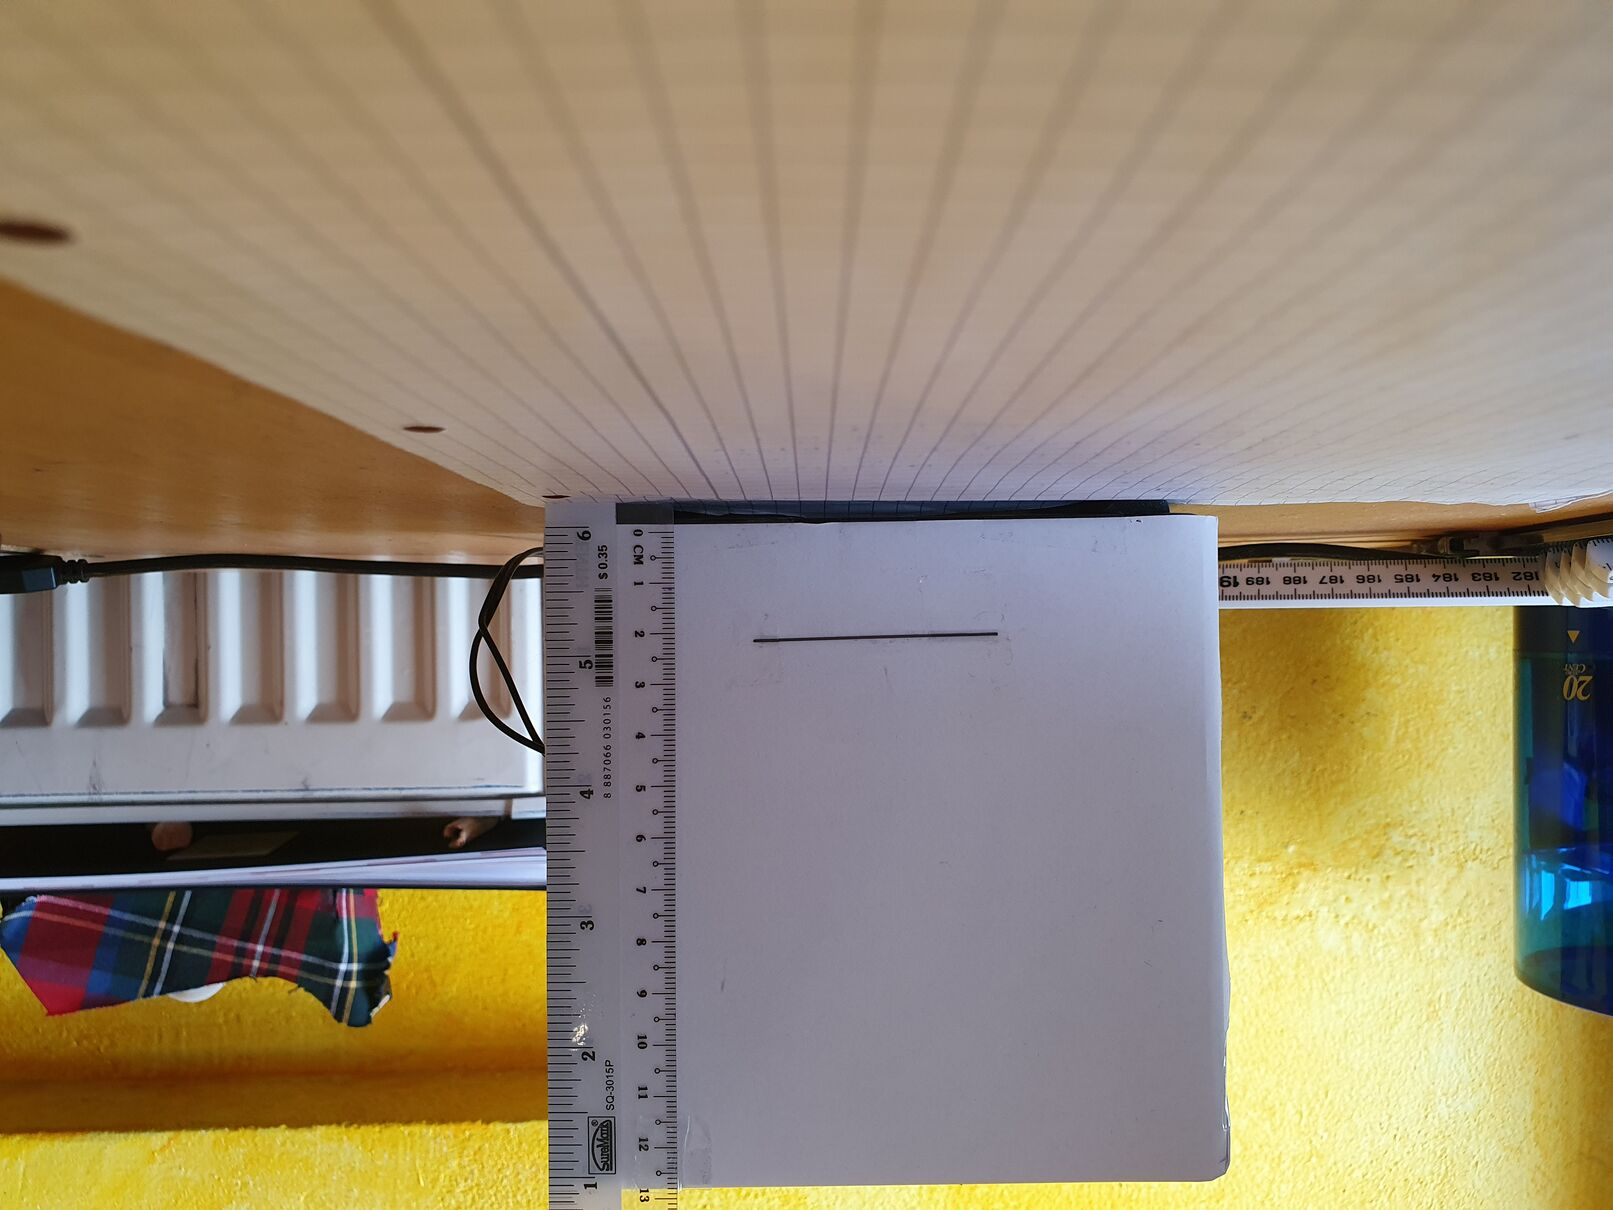
\includegraphics[width=0.6\textwidth,angle=180,origin=c]{images/tv3/eye.jpg}
				\caption{Augensicht, Bild zur Auswertung, komprimiert}
				\label{fig:tv3-data-eye}
				\vspace{-10pt}
			\end{figure}
		% \vspace{0.5\baselineskip}
		\underline{\large\textit{Foldscope}}
		\vspace{0.5\baselineskip}

			\begin{figure}[H]
				\centering
				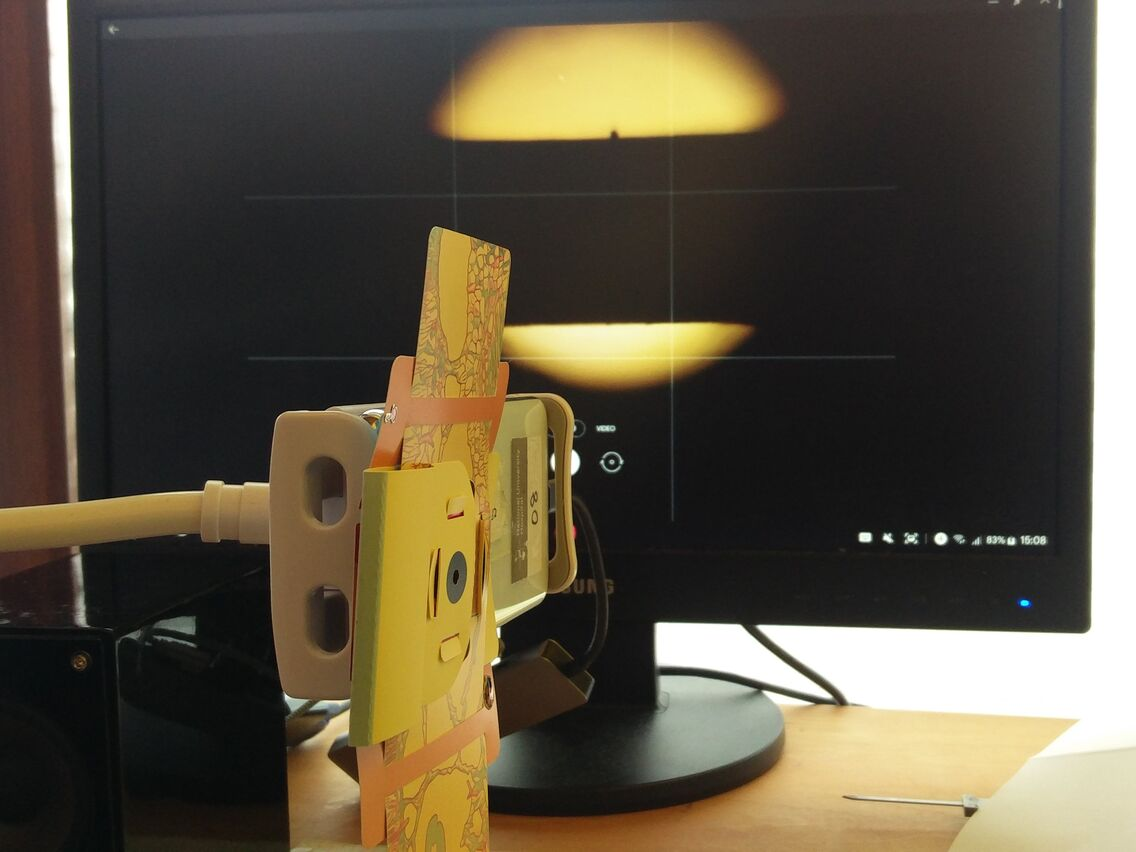
\includegraphics[width=0.65\textwidth]{images/tv3/tv3-aufbau-03.jpg}
				\caption{Aufbau fürs Foldscope}
				\label{fig:tv3-nah-aufbau}
				\vspace{-15pt}
			\end{figure}
			Für die Sicht aus dem Foldscope wurde der dritte Magnetkoppler auf dem Handy mit Klebeband geklebt. Die Vorbereitung der Präparate erfolgt wie im Teilversuch \ref{sec:tv2}. Um das Bild konstant zu halten wurde das Handy mit dem Foldscope auf einem Handyhalter befestigt. 

			Das Foldscope wurde dann so rotiert, dass die Bleistiftmine horizontal im Bild steht. Mit dem Fokusteil des Foldscopes wurde das Kamera auf dem Zentrum vom Bild fokussiert. Das Foto wurde wieder durch die Kamera-App im Samsung DeX aufgenommen, um alle Faktoren konstant zu halten. 

			Als Messdaten haben wir das Bild:
			\begin{figure}[H]
				\centering
				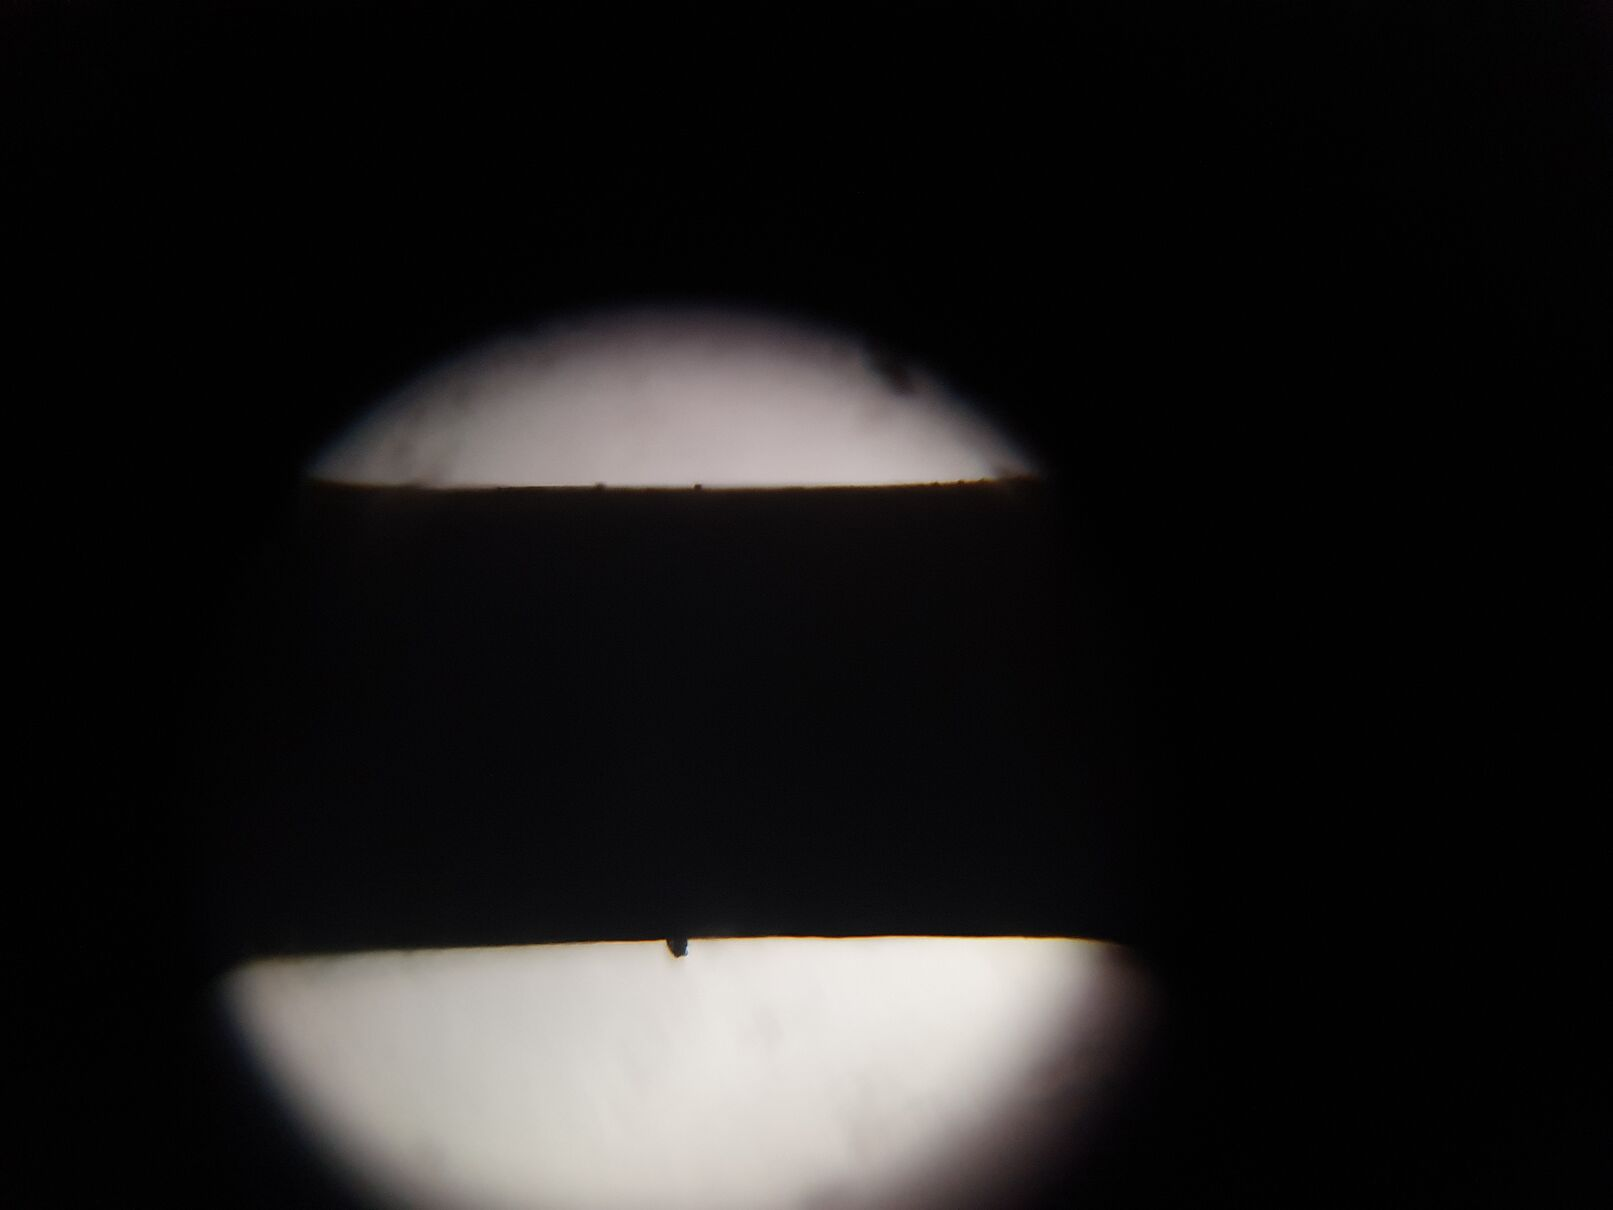
\includegraphics[width=0.6\textwidth,angle=180,origin=c]{images/tv3/foldscope.jpg}
				\caption{Sicht aus dem Foldscope, Bild zur Auswertung, komprimiert}
				\label{fig:tv3-data-scope}
				\vspace{-10pt}
			\end{figure}
			\newpage
	\subsection{Auswertung}
		Um die relative Bildhöhe zwischen Abbildung \ref{fig:tv3-data-eye} und Abbildung \ref{fig:tv3-data-scope} zu bestimmen haben wir das Programm GIMP 2.10.22\footnote{\url{https://www.gimp.org/}} verwendet. 
		\begin{figure}[H]
			\centering
			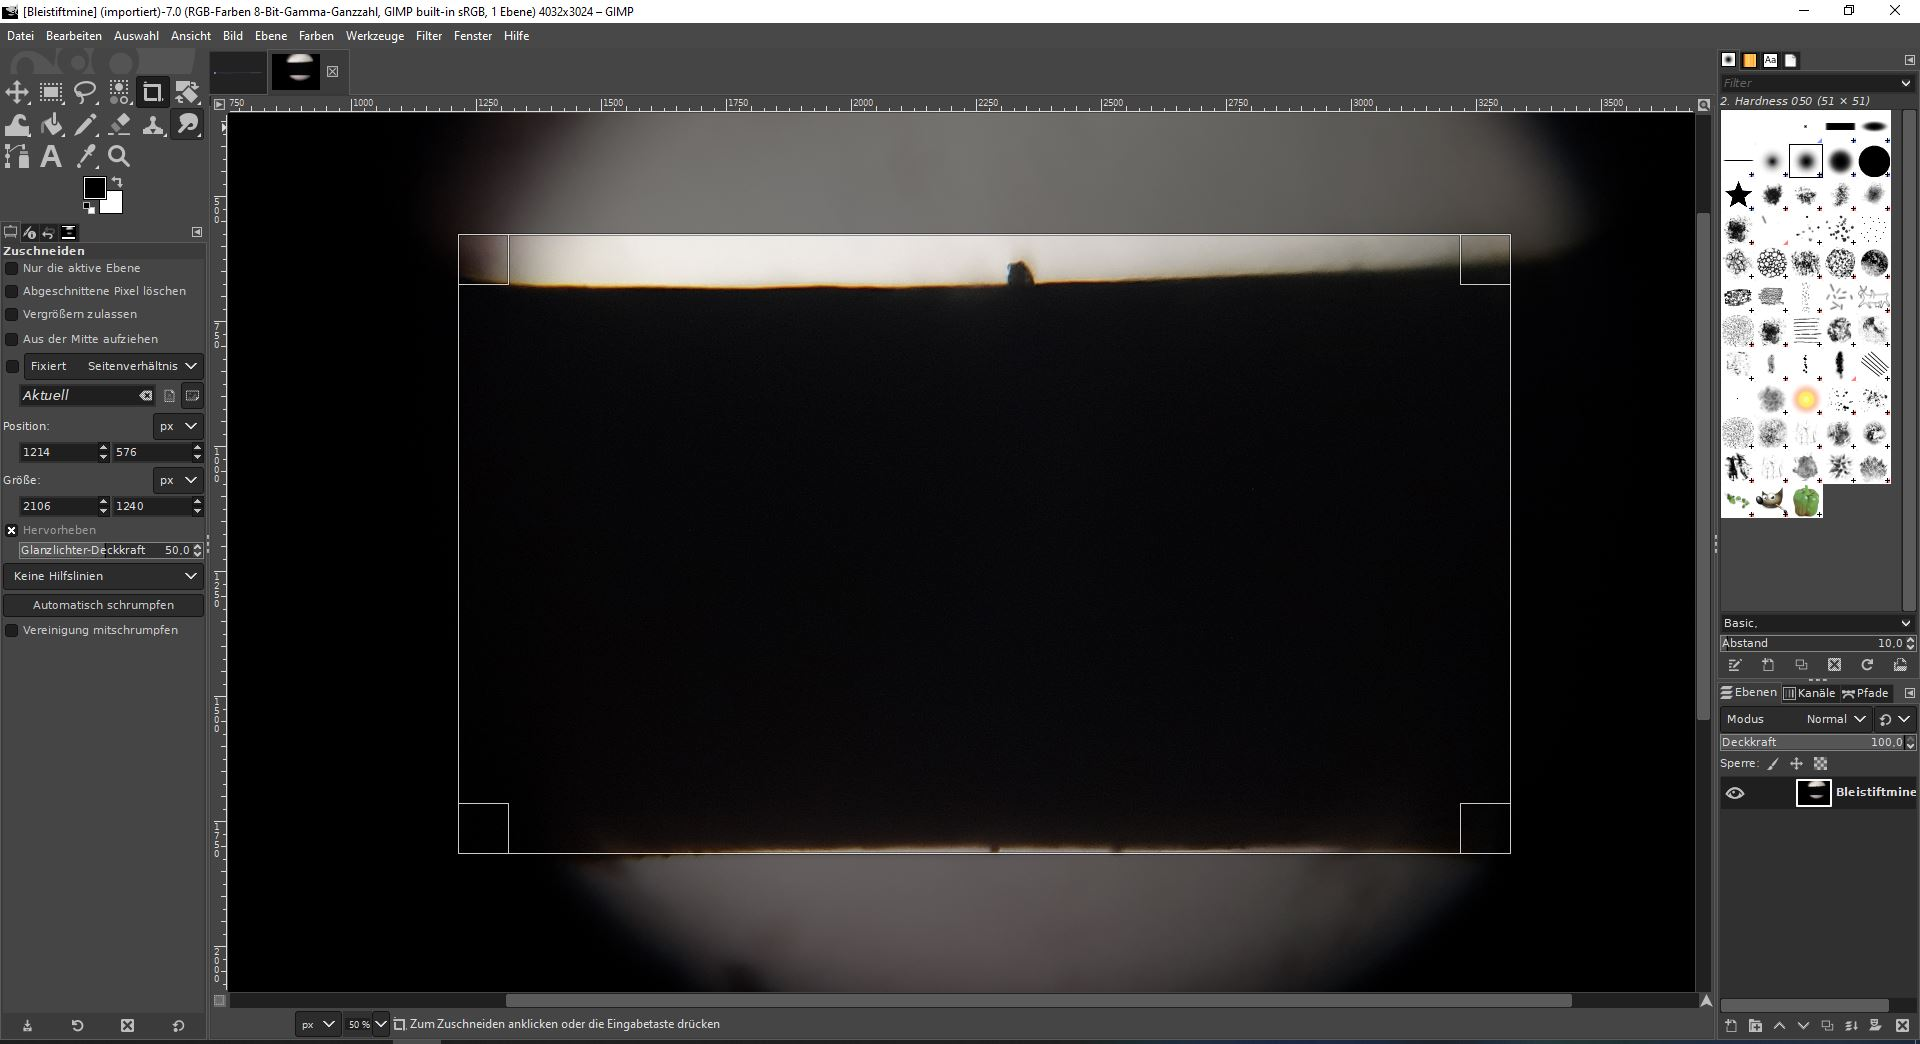
\includegraphics[width=0.8\textwidth]{images/tv3/cropping.jpg}
			\caption{Grobe Zuschneiden von Bildern im GIMP}
			\vspace{-10pt}
		\end{figure}
		Es wurde immer den Teil der Bleistiftmine ausgeschnitten. Die resultierende Anzahl der vertikalen Pixels ist dann die Bildhöhe. Zur Fehlerbestimmung haben wir bei der Gradient am Rand der Bleistiftmine eine obere und untere Grenze abgeschätzt. Wo nötig haben wir das Bild so gedreht, dass die Bleistiftmine im Bild horizontal steht.

		Als Messwerten haben wir:
		\begin{center}
			\vspace{\baselineskip}
			\begin{tabular}{llll}
				\toprule
				Sicht & Max $/$ \si{\pixel} & Min $/$ \si{\pixel} & Bildhöhe $/$ \si{\pixel}  \\
				\midrule
				Bloße Augen $B_e$ & \num{8} & \num{6} & \num{7(1)} \\
				Foldscope  $B_f$ & \num{1128} & \num{1108} & \num{1118(10)} \\
				\bottomrule
			\end{tabular}
			\vspace{\baselineskip}
		\end{center}
		Aus der Anleitung ist die Vergrößerung (und deren Fehler) gegeben durch:
		\begin{align}
			\Gamma &= \frac{B_f}{B_e} = \frac{\SI{1118}{\pixel}}{\SI{7}{\pixel}} = \num{159.714} \sigfig{6} \\
			\Delta\Gamma &= \gamma\relquad{B_f,B_e} = \left(\frac{1118}{7}\right)\sqrt{
				\left(\frac{1}{7}\right)^2 +
				\left(\frac{10}{1118}\right)^2
				} \notag \\
				&= \num{23} \sigfig{2}
		\end{align}
		Somit erhalten wir als experimentelle Wert eine Vergrößerung von $\Gamma_\text{exp} = \num{160(23)}$.

		Die theoretische Vergrößerung (und deren Fehler) ist laut der Anleitung gegeben durch:
		\begin{align}
			\Gamma &= \frac{l}{f} \overset{\eqref{eqn:focallength}}{=} l \left(\frac{4(n-1)}{nD}\right) = \frac{4l(n-1)}{nD} \notag \\
			&= \frac{4l}{D}\left(\frac{n-1}{n}\right) = \frac{4l}{D}\left(1-\frac{1}{n}\right) \\
			\Delta\Gamma &= \gausserror{\Gamma}{l,n}
		\end{align}
		da $D$ ohne Fehler gegeben ist. 

		Mit
		\begin{align}
			\pdv{\Gamma}{l} = \frac{4}{D}\left(1-\frac{1}{n}\right) && \pdv{\Gamma}{n} = \frac{4l}{Dn^2}
		\end{align}
		ist der Fehler $\Delta\Gamma$ gegeben durch:
		\begin{align}
			\Delta\Gamma = \frac{4l}{D}\sqrt{\left(1-\frac{1}{n}\right)^2\left(\frac{\Delta l}{l}\right)^2 + \left(\frac{\Delta n}{n^2}\right)^2}
			\label{eqn:delta-gamma}
		\end{align}
		Mit $n = \frac{n_L}{n_M}$ ist 
		\begin{align}
			\Delta n = \frac{n_L}{n_M}\relquad{n_L, n_M}
			\label{eqn:delta-n}
		\end{align}
		Der sichtbare Bereich der menschlichen Augen ist zwischen \SI{380}{\nano\meter} und \SI{750}{\nano\meter} \citep{starr_biology_2006}. In diesem Bereich ist der Brechungsindex von Luft $n_M = \num{1.0003}$ relativ konstant\footnote{\url{https://refractiveindex.info/?shelf=other&book=air&page=Ciddor}}. Man kann somit $n_M$ als fehlerfrei betrachten. Das ist aber nicht der Fall für den Brechungsindex von Borsilikatglas (BK7 oder manchmal auch N-BK7):
		\begin{figure}[H]
			\centering
			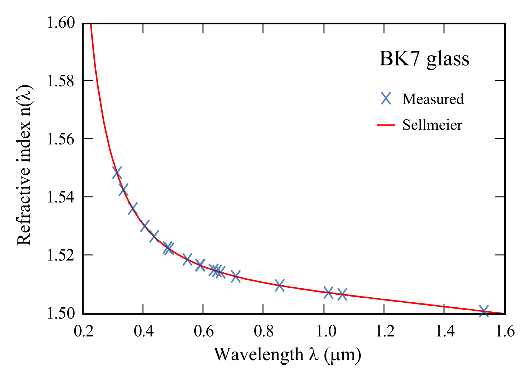
\includegraphics[width=0.6\textwidth]{plots/bk7.eps}
			\caption{\centering Brechungsindex von BK7 \\ (\textit{File:Sellmeier-equation.svg}, Autor: Wikipedia Benutzer \textit{DrBob} \ccbysa)}
		\end{figure}
		Ideal wäre, wenn wir die Intensitätverteilung wissen und daraus die mittlere Brechungsindex von BK7 berechnen. Da wir aber weder den Hersteller der Linse noch die Intensitätverteilung der Lichtquelle wissen, ist der einfache Mittelwert (mit entsprechender Schwankung als Fehler) eine vernünftige Annahme hier. Der Verlauf der Brechungsindex im sichbaren Bereich ist hier auch als eine lineare Verlauf genähert. 

		Wir gehen auch davon aus, dass die Temperatur keinen Einfluss hat. 

		Im sichtbaren Bereich hat N-BK7 von SCHOTT\footnote{\url{https://refractiveindex.info/?shelf=glass&book=BK7&page=SCHOTT}}:
		\begin{equation}
			\begin{split}
				n_\text{max} &= \num{1.5337} \text{ bei } \SI{380}{\nano\meter} \\
				n_\text{min} &= \num{1.5118} \text{ bei } \SI{750}{\nano\meter}
			\end{split}
		\end{equation}
		Somit ist $n_L$ gegeben durch
		\begin{align}
			n_L &= \frac{\num{1,5337} + \num{1,5118}}{2} = \num{1.52275} \\
			\Delta n_L &= \frac{\num{1,5337} - \num{1,5118}}{2} = \num{0.011} \sigfig{2}
		\end{align}
		Also ist $n_L = \num{1.523(11)}$ und es gilt nach Gleichung \eqref{eqn:delta-n}:
		\begin{align}
			\Delta n = \frac{\cancel{n_L}}{n_M}\left(\frac{\Delta n_L}{\cancel{n_L}}\right) = \frac{\Delta n_L}{n_M}
			\label{eqn:real-delta-n}
		\end{align}
		Die Gleichung \eqref{eqn:delta-gamma} ist dann
		\begin{align}
			\Delta\Gamma &= \frac{4l}{D}\sqrt{\left(1-\frac{1}{n}\right)^2\left(\frac{\Delta l}{l}\right)^2 + \left(\frac{\Delta n}{n^2}\right)^2} \notag \\
			&= \frac{4l}{D}\sqrt{
				\left(1-\frac{n_M}{n_L}\right)^2\left(\frac{\Delta l}{l}\right)^2 
				+ \left(\frac{\Delta n_L}{n_M}\left(\frac{n_M}{n_L}\right)^2\right)^2
			} \notag \\
			&= \frac{4l}{D}\sqrt{
				\left(1-\frac{n_M}{n_L}\right)^2\left(\frac{\Delta l}{l}\right)^2 
				+ \left(n_M\frac{\Delta n_L}{n_L^2}\right)^2
			}
			\label{eqn:real-gamma-error}
		\end{align}
		Der Fehler der Brennweite (Gleichung \eqref{eqn:focallength}), was auch gefragt wird, ist dann gegeben durch:
		\begin{align}
			\Delta f &= \gausserror{f}{n} = \abs{\frac{D(\Delta n)}{4}\pdv{}{n}\left(\frac{n}{n - 1}\right)} = \abs{\frac{D(\Delta n)}{4}\pdv{}{n}\left(1+\frac{1}{n - 1}\right)} \notag \\
			{\scriptsize \eqref{eqn:real-delta-n}} &= 
				\frac{D(\Delta n_L)}{4n_M}\frac{1}{(n-1)^2} 
				= \frac{D(\Delta n_L)}{4n_M}\left(\frac{n_M}{n_L - n_M}\right)^2 \notag \\
				&=\frac{Dn_M(\Delta n_L)}{4(n_L - n_M)^2}
			\label{eqn:real-f-error}
		\end{align}
		\newpage
		Mit der Werten
		\begin{center}
			\begin{tabular}{lll}
				\toprule
				Variable & Wert & Bedeutung \\
				\midrule
				$D$ & \SI{2.38}{\milli\meter} & Durchmesser der Kugellinse \\
				$n_M$ & \num{1.0003} & Brechungsindex von Luft \\
				$n_L$ & \num{1.523(11)} & Brechungsindex von BK7 \\
				$l$ & \SI{0.250(1)}{\meter} & Deutliche Sehweite (im Experiment) \\
				\bottomrule
			\end{tabular}
		\end{center}
		ist die Vergrößerung gegeben durch:
		\begin{align}
			\Gamma &= \frac{4l}{D}\left(1-\frac{n_M}{n_L}\right) = \frac{4(\SI{0.250}{\meter})}{\SI{2.38e-3}{\meter}}\left(1-\frac{\num{1.0003}}{\num{1.523}}\right) \notag \\
			&= \num{144.203} \sigfig{6} \\
			\Delta \Gamma &= \frac{4(\SI{0.250}{\meter})}{\SI{2.38e-3}{\meter}}\notag \\
			&\phantom{=}\times\sqrt{
				\left(1-\frac{\num{1.0003}}{\num{1.523}}\right)^2\left(\frac{0.001}{0.250}\right)^2 
				+ \left(\frac{(\num{1.0003})(0.011)}{(1.523)^2}\right)^2
			} \notag \\
			&= \num{2.1} \sigfig{2}
		\end{align}
		Somit erhalten wir $\Gamma_\text{theo} = \num{144.2(21)}$.

		Die Brennweite ist mit der gleichen Werten gegeben durch:
		\begin{align}
			f &= \frac{nD}{4(n-1)} = \frac{D}{4}\left(1 + \frac{n_M}{n_L - n_M}\right) \notag \\
			&= \frac{\SI{2.38e-3}{\meter}}{4}\left(1 + \frac{\num{1.0003}}{\num{1.523} - \num{1.0003}}\right) \notag \\
			&= \SI{1.73366}{\milli\meter} \sigfig{6} \\
			\Delta f &= \frac{Dn_M(\Delta n_L)}{4(n_L - n_M)^2} 
			= \frac{(\SI{2.38e-3}{\meter})(\num{1.0003})(\num{0.011})}{4(1.523 - 1.0003)^2} \notag \\
			&= \SI{2.4e-2}{\milli\meter} \sigfig{2}
		\end{align}
		Somit erhalten wir $f = \SI{1.734(24)}{\milli\meter}$.

	\subsection{Diskussion}
		Als Endergebnisse erhalten wir:
		\begin{center}
			\begin{tabular}{lll}
				\toprule
				Experimentell & $\Gamma_\text{exp}$ & \num{160(23)} \\
				Theoretisch & $\Gamma_\text{theo}$ & \num{144.2(21)} \\
				\bottomrule
			\end{tabular}
		\end{center}
		Die Werten stimmen also miteinander überein, da die Fehlerintervalle sich überschneiden. Es gibt aber hier wegen der Auflösung der Kamera eine große Unsicherheit bei dem experimentellen Wert.

		Außerdem sehen wir -- besonders im Teilversuch 2 (Abbildung \ref{fig:tv2-proben}) -- auch zusätzlich zur sphä\-rischen Abberationen chromatische Abberationen. Diese kann man mit der großen Wel\-len\-län\-ge\-ab\-hän\-gig\-keit des Brechungsindex von BK7 im sichrbaren Bereich gut erklären. 

		Es ist vielleicht auch interessant zu bemerken, dass die Brennweite ($f = \SI{1.734(24)}{\milli\meter}$) ungefähr die Hälfte der Höhe des Fokusteils entspricht (etwa \SI{4}{\milli\meter}). 

	\subsection{Unterschied mit klassichen Mikroskopen}
		In klassichen Mikroskopen befindet sich normalerweise mindestens 2 Linsen, die ein optisches System bildet anstatt eine, die wir im Foldscope haben. Es gibt auch oft fast keine Abberationen zu beobachten, da diese durch das Linsensystem unterdruckt sind, sodass man Proben gut untersuchen kann. 

		Außer des optisches System ist die Steuerung des klassichen Mikroskops viel feiner als die des Foldscopes. Man hat auch bei gutem Mikroskopsystemen die Wahl zwischen Lichtfeld- und Dunkelfeldmikroskopie. Es gibt auch normalerweise eine Wahl zwischen verschiedene Vergrößerungen, was man mit einem Foldscope nicht hat. 

		Obwohl die klassiche Mikroskopen deswegen viele Vorteile haben, ist die Kosten eines klassichen Mikroskops. 